\subsection{Módulo NFC}

Para su desarrollo, hemos utilizado el periférico I2C1, el protocolo RF, la placa \texttt{ANT7-T-M24SR64} \cite{M24SR64YPagWeb} de ST Microelectronics y la aplicación móvil **NFC Tools** \cite{NFCTools}. Además, a la hora de realizar comprobaciones desarrollando el módulo, hemos utilizado la app \texttt{ST25} \cite{ST25}.

\texttt{ANT7-T-M24SR64}: 
La placa \texttt{ANT7-T-M24SR64} es una placa que incluye un \texttt{M24SR64-Y}. \texttt{M24SR64-Y} es una tag dinámica NFC/RFID, EEPROM de interfaz dual, con protocolos RF e I2C. Se puede operar desde una interfaz I2C, un lector RFID o un teléfono con NFC.

Figura 1: \texttt{ANT7-T-M24SR64} [M24SR.png]
\begin{figure}[h]
    \centerin
    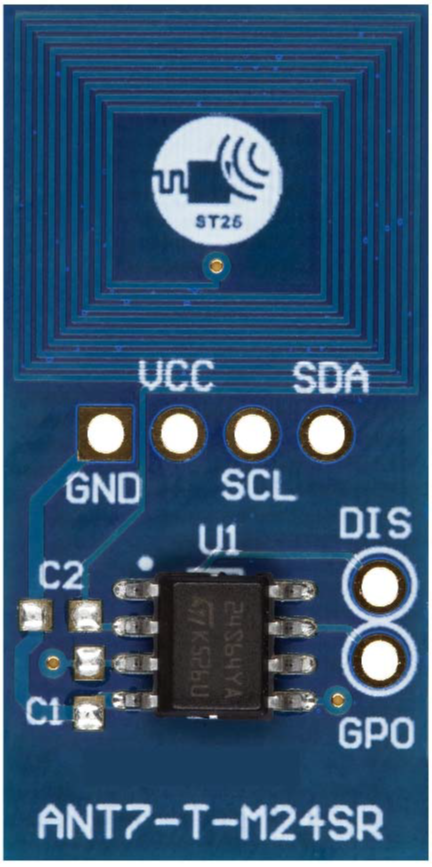
\includegraphics[width=0.5\textwidth]{images/2/2-5/M24SR.png}
    \caption{Módulo NFC \texttt{ANT7-T-M24SR64}}
    \label{fig:2-5-modulo-nfc}
\end{figure}

Como se puede observar en la figura anterior, hay 6 pines:

- \texttt{VCC}: Alimentación 3.3 V.
- \texttt{GND}: Masa.
- \texttt{SDA}: Línea de datos del bus I2C.
- \texttt{SCL}: Señal de reloj del bus I2C.
- \texttt{GPO}: A nivel bajo, RF o I2C está siendo utilizado. A nivel alto, está libre.
- \texttt{DIS}: Activación/Desactivación de los comandos RF.
